\documentclass[portrait,final,a0paper]{baposter}
%\documentclass[a4shrink,portrait,final]{baposter}
% Usa a4shrink for an a4 sized paper.

\tracingstats=2

\usepackage{calc}
\usepackage{graphicx}
\usepackage{amsmath}
\usepackage{amssymb}
\usepackage{relsize}
\usepackage{multirow}
\usepackage{bm}

\usepackage{graphicx}
\usepackage{multicol}

\usepackage{pgfbaselayers}
\pgfdeclarelayer{background}
\pgfdeclarelayer{foreground}
\pgfsetlayers{background,main,foreground}

\usepackage{times}
\usepackage{helvet}
%\usepackage{bookman}
\usepackage{palatino}

\newcommand{\captionfont}{\footnotesize}

\selectcolormodel{cmyk}

\graphicspath{{images/}}

%%%%%%%%%%%%%%%%%%%%%%%%%%%%%%%%%%%%%%%%%%%%%%%%%%%%%%%%%%%%%%%%%%%%%%%%%%%%%%%%
%%%% Some math symbols used in the text
%%%%%%%%%%%%%%%%%%%%%%%%%%%%%%%%%%%%%%%%%%%%%%%%%%%%%%%%%%%%%%%%%%%%%%%%%%%%%%%%
% Format 
\newcommand{\Matrix}[1]{\begin{bmatrix} #1 \end{bmatrix}}
\newcommand{\Vector}[1]{\Matrix{#1}}
\newcommand*{\SET}[1]  {\ensuremath{\mathcal{#1}}}
\newcommand*{\MAT}[1]  {\ensuremath{\mathbf{#1}}}
\newcommand*{\VEC}[1]  {\ensuremath{\bm{#1}}}
\newcommand*{\CONST}[1]{\ensuremath{\mathit{#1}}}
\newcommand*{\norm}[1]{\mathopen\| #1 \mathclose\|}% use instead of $\|x\|$
\newcommand*{\abs}[1]{\mathopen| #1 \mathclose|}% use instead of $\|x\|$
\newcommand*{\absLR}[1]{\left| #1 \right|}% use instead of $\|x\|$

\def\norm#1{\mathopen\| #1 \mathclose\|}% use instead of $\|x\|$
\newcommand{\normLR}[1]{\left\| #1 \right\|}% use instead of $\|x\|$

\def\bi{\begin{itemize}}
\def\ei{\end{itemize}}
\def\im{\item}

%%%%%%%%%%%%%%%%%%%%%%%%%%%%%%%%%%%%%%%%%%%%%%%%%%%%%%%%%%%%%%%%%%%%%%%%%%%%%%%%
% Multicol Settings
%%%%%%%%%%%%%%%%%%%%%%%%%%%%%%%%%%%%%%%%%%%%%%%%%%%%%%%%%%%%%%%%%%%%%%%%%%%%%%%%
\setlength{\columnsep}{0.7em}
\setlength{\columnseprule}{0mm}


%%%%%%%%%%%%%%%%%%%%%%%%%%%%%%%%%%%%%%%%%%%%%%%%%%%%%%%%%%%%%%%%%%%%%%%%%%%%%%%%
% Save space in lists. Use this after the opening of the list
%%%%%%%%%%%%%%%%%%%%%%%%%%%%%%%%%%%%%%%%%%%%%%%%%%%%%%%%%%%%%%%%%%%%%%%%%%%%%%%%
\newcommand{\compresslist}{%
\setlength{\itemsep}{1pt}%
\setlength{\parskip}{0pt}%
\setlength{\parsep}{0pt}%
}


%%%%%%%%%%%%%%%%%%%%%%%%%%%%%%%%%%%%%%%%%%%%%%%%%%%%%%%%%%%%%%%%%%%%%%%%%%%%%%
%%% Begin of Document
%%%%%%%%%%%%%%%%%%%%%%%%%%%%%%%%%%%%%%%%%%%%%%%%%%%%%%%%%%%%%%%%%%%%%%%%%%%%%%

\begin{document}

%%%%%%%%%%%%%%%%%%%%%%%%%%%%%%%%%%%%%%%%%%%%%%%%%%%%%%%%%%%%%%%%%%%%%%%%%%%%%%
%%% Here starts the poster
%%%---------------------------------------------------------------------------
%%% Format it to your taste with the options
%%%%%%%%%%%%%%%%%%%%%%%%%%%%%%%%%%%%%%%%%%%%%%%%%%%%%%%%%%%%%%%%%%%%%%%%%%%%%%
% Define some colors

\definecolor{yellow}{cmyk}{0,0,0.9,0.0}
\definecolor{reddishyellow}{cmyk}{0,0.22,1.0,0.0}
\definecolor{black}{cmyk}{0,0,0.0,1.0}
\definecolor{darkYellow}{cmyk}{0,0,1.0,0.5}
\definecolor{lightyellow}{cmyk}{0,0,0.3,0.0}
\definecolor{lighteryellow}{cmyk}{0,0,0.1,0.0}
\definecolor{lighteryellow}{cmyk}{0,0,0.1,0.0}
\definecolor{lightestyellow}{cmyk}{0,0,0.05,0.0}

\definecolor{silver}{cmyk}{0,0,0,0.3}
\definecolor{lightsilver}{cmyk}{0,0,0,0.15}
\definecolor{lightersilver}{cmyk}{0,0,0,0.10}
\definecolor{lightestsilver}{cmyk}{0,0,0,0.01}
\definecolor{darkSilver}{cmyk}{0,0,0,0.1}
\definecolor{white}{cmyk}{0,0,0,0}
\definecolor{darkblue}{cmyk}{0.93,0.93,0,0.78}
\definecolor{blue}{cmyk}{0.53,0.53,0,0.62}
\definecolor{h-alpha-2}{cmyk}{0,0.05,0.02,0.17}

%%
\typeout{Poster Starts}
\background{
  \begin{tikzpicture}[remember picture,overlay]%
    \draw (current page.north west)+(-2em,2em) node[anchor=north west] {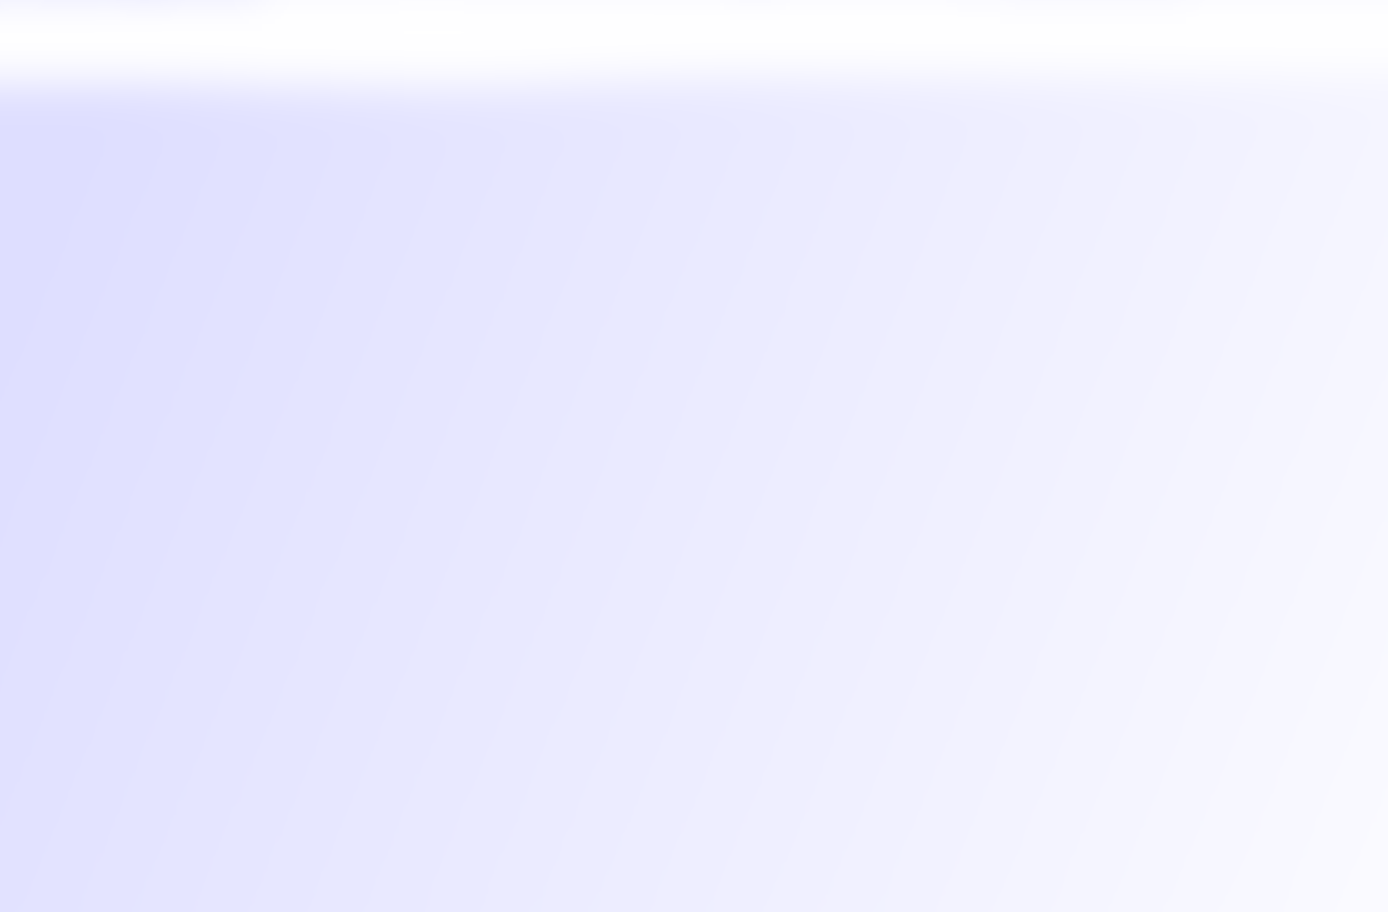
\includegraphics[height=1.1\textheight]{silhouettes_background}};
  \end{tikzpicture}%
}

\newlength{\leftimgwidth}
\begin{poster}%
  % Poster Options
  {
  % Show grid to help with alignment
  grid=no,
  % Column spacing
  colspacing=1em,
  %%Ondra G modra
  %%
  %bgColorOne=white,  %First background color. There are two background color to allow for background gradients.
  %bgColorTwo=lightestsilver,
  %borderColor=h-alpha-2,		%Color used for the borders of the poster boxes
  %headerColorTwo=darkblue,	%First color of box header. Two colors can be used to dene gradients.
  %headerColorOne=blue,
  %headerFontColor=white,
  %boxColorOne=h-alpha-2,
  %boxColorTwo=white,
%=%========== barevné přechody==========
 %% Format of textbox
% %==========nové ===============
  %textborder=roundedleft,  %Which kind of border should the lower part of the text boxes have. Possible values are:
  %  		    %1. none 2. bars 3. coils 4. triangles 5. rectangle 6. rounded 7. faded
  %% Format of text header
  %headerborder=open,%At which sides of the text box headers should we draw a border. Possible values are:
  %  	    %1. none 2. closed 3. open
  %headershape=roundedright,
  %headershade=shade-tb, %1. plain 2. shade-lr 3. shade-tb 4. shade-tb-inverse
  %boxshade=shade-lr,
  %background=plain,

  % Color style
%  ============žlutá ==============
%   bgColorOne=lighteryellow,
%   bgColorTwo=lightestyellow,
%   borderColor=reddishyellow,
%   headerColorOne=yellow,
%   headerColorTwo=reddishyellow,
%   headerFontColor=black,
%   boxColorOne=lightyellow,
%   boxColorTwo=lighteryellow,
% ============stříbrná ==============
  bgColorOne=lightersilver,  %First background color. There are two background color to allow for background gradients.
  bgColorTwo=lightestsilver,
  borderColor=silver,		%Color used for the borders of the poster boxes
  headerColorOne=silver,	%First color of box header. Two colors can be used to dene gradients.
  headerColorTwo=lightersilver,
  headerFontColor=black,
  boxColorOne=lightestsilver,
  boxColorTwo=white,
%=========== barevné přechody==========
 % Format of textbox
% ==========nové ===============
  textborder=roundedleft,  %Which kind of border should the lower part of the text boxes have. Possible values are:
  %  		    %1. none 2. bars 3. coils 4. triangles 5. rectangle 6. rounded 7. faded
  %% Format of text header
  headerborder=open,%At which sides of the text box headers should we draw a border. Possible values are:
  %  	    %1. none 2. closed 3. open
  headershape=roundedright,
  headershade=shade-tb, %1. plain 2. shade-lr 3. shade-tb 4. shade-tb-inverse
  boxshade=shade-lr,
  background=shade-tb,
%==========původní ===============
%   % Format of textbox
%   textborder=roundedleft,
%   % Format of text header
%   headerborder=open,
%   headershape=roundedright,
%   headershade=plain,
%   boxshade=plain,
%   background=plain,
% zbytek
  headerfont=\Large\textsf, %Sans Serif
  headerheight=0.12\textheight,%Height of the main poster header (not of the headers of the text boxes).
  eyecatcher=yes,
  linewidth=2pt
  }
  % Eye Catcher
  {
\includegraphics[width=7em]{golem.pdf}} % No eye catcher for this poster. (eyecatcher=no above). If an eye catcher is present, the title is centered between eye-catcher and logo.
  % Title
  {%\sf %Sans Serif
  \sc\huge    The Tokamak GOLEM for Fusion Education \vspace{ 0.2cm}}
  % Authors
  {%Sans Serif
  % Serif
  E. Bromov\'a$^1$, I. \v Duran$^2$, O. Grover$^1$, J. Kocman$^1$, T. Markovi\v{c}$^1$, M. Odstr\v cil$^{12}$, T.\,Odstr\v cil$^1$\!, O.\,Pluha\v r$^3$\!, J.\,St\" ockel$^2$\!, V.\,Svoboda$^1$\!, A.\,\v Sindlery$^1$\!, G.\,Vondr\'a\v sek$^1$\!, J.\,Zara$^3$\!.\\
{\large $^1$Faculty of Nuclear Sciences and Physical Engineering CTU Prague, CZ-115 19, Czech Rep.\\$^2$Institute of Plasma Physics AS CR, CZ-182 21 Prague, Czech Republic.\\$^3$Faculty of Electrical Engineering CTU Prague, CZ-166 27, Czech Rep.}
}{
    \makebox[8em][r]{%
      \begin{minipage}{8em}
	
\includegraphics[width=7em]{lev}\\~\\
        
\includegraphics[width=7em]{logoipp}
      \end{minipage}}
}


%%%%%%%%%%%%%%%%%%%%%%%%%%%%%%%%%%%%%%%%%%%%%%%%%%%%%%%%%%%%%%%%%%%%%%%%%%%%%%
%%% Now define the boxes that make up the poster
%%%---------------------------------------------------------------------------
%%% Each box has a name and can be placed absolutely or relatively.
%%% The only inconvenience is that you can only specify a relative position 
%%% towards an already declared box. So if you have a box attached to the 
%%% bottom, one to the top and a third one which should be in between, you 
%%% have to specify the top and bottom boxes before you specify the middle 
%%% box.
%%%%%%%%%%%%%%%%%%%%%%%%%%%%%%%%%%%%%%%%%%%%%%%%%%%%%%%%%%%%%%%%%%%%%%%%%%%%%%
%%%%%%%%%%%%%%%%%%%%%%%%%%%%%%%%%%%%%%%%%%%%%%%%%%%%%%%%%%%%%%%%%%%%%%%%%%%%%%
\headerbox{The GOLEM Tokamak}{name=GOLEMtokamak,column=0,row=0}
{
  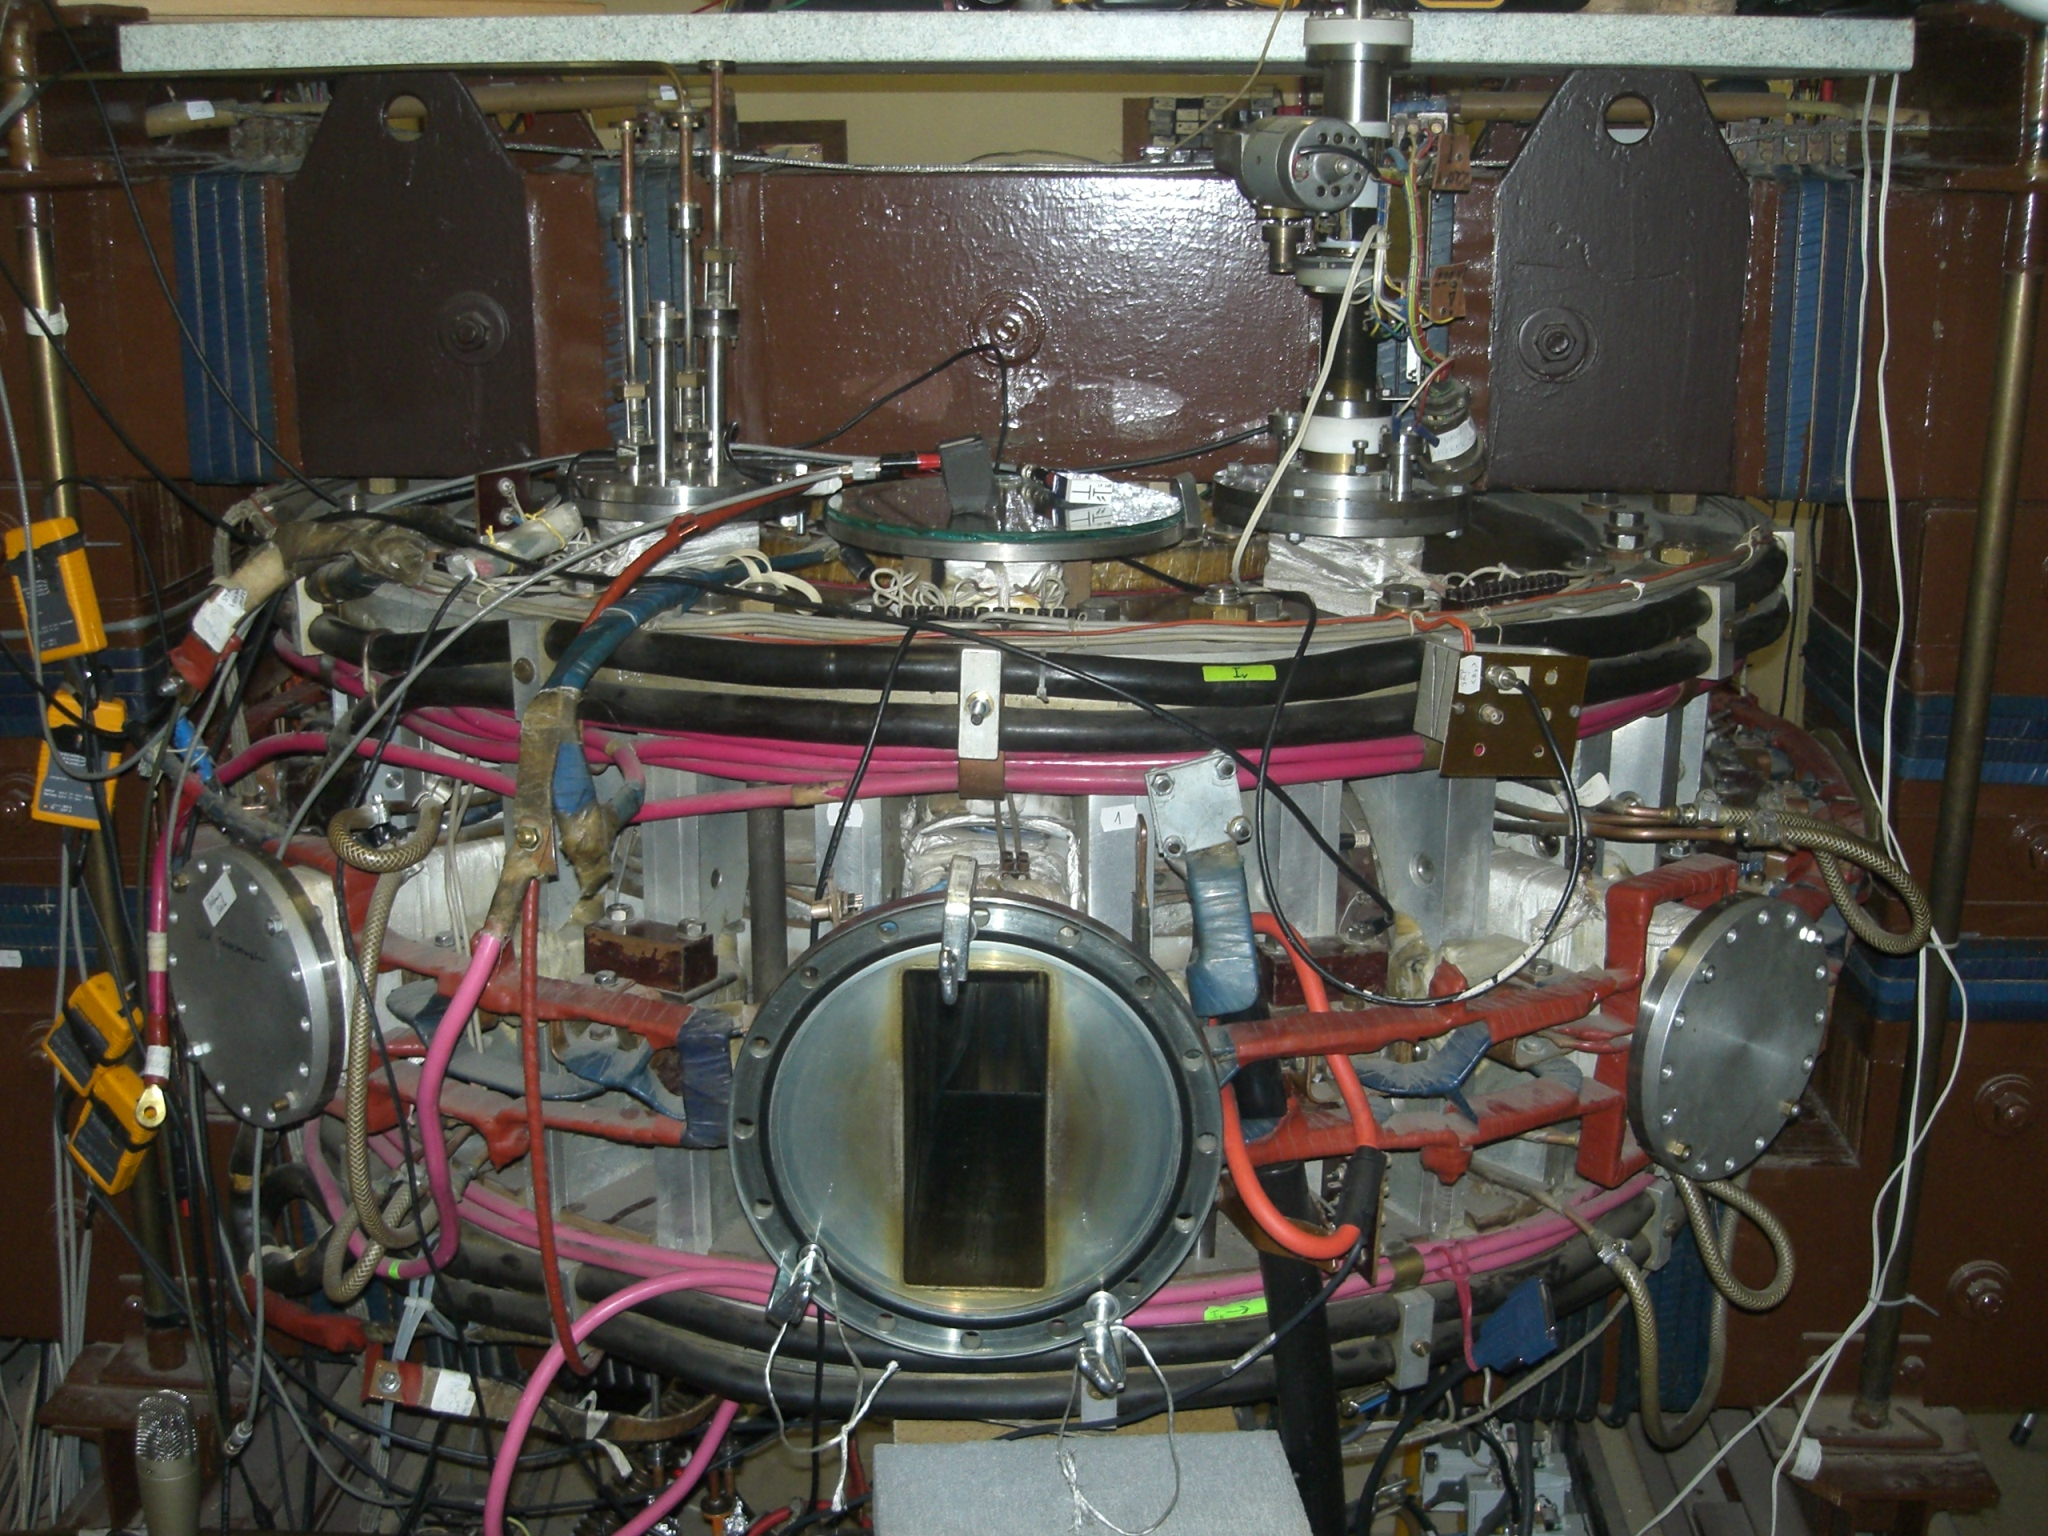
\includegraphics[width=\textwidth]{cimg8714.jpg}
%   \begin{list}{\labelitemi}{\itemsep=-2pt \topsep=-2pt}
\bi
    \im An educational device for domestic as well as for foreign students via remote participation/handling.
        \im Operating routinely for nearly two years at a modest range of parameters $B_t < 0.5$ T, $I_p < 8$ kA, pulse length $< 15$ ms, and with a limited set of diagnostics. 
    \im Wide range of tasks with varying levels of complexity covering tokamak physics, technology and operation can be studied by the future fusion specialists.
%   \end{list}
\ei
 }

\headerbox{Recent Diagnostics Enrichment - Students' Contribution}{name=latterdiagnostics,column=1,row=0, span=2}
{
  \def\contr#1#2#3#4#5{
  \begin{minipage}{0.48\textwidth}
%   \begin{center}
  {\bf #1}\\
  { #2}
  \includegraphics[width=#4\textwidth,height=!]{#3}
  {\it { #5}}
%   \end{center}
  \end{minipage}}
\begin{multicols}{2}
 \contr{Electron Density Measurement}{The oldest and most widespread MW diagnostics is now implemented at the GOLEM tokamak. A generated MW interacts with the magnetized plasma which results in a change of the MW's phase. Interferometry evaluates the MW signal that has passed through plasma relative to the reference signal.}{density}{1}{Evolution of a typical Golem discharge. The loop voltage, toroidal magnetic field, plasma current, signal of a photodiode, and newly the electron density measurement.}
\medskip

    \contr{High Speed VIS Cameras}{Two cameras Casio EX-F1 have been installed in ports at one poloidal cross-section  perpendicular to the plasma column. This configuration is suitable for VIS tomography. The camera can achieve frame rate up to 1200\,fps, however the real time resolution is up to 40\,kHz because of the ``rolling shutter effect''.}{plasma-HS-camera-image2}{1}{{ Plasma column observed from the horizontal port \, during shot \#3754, exposure time $50\,\mu$s}}

 \contr{Plasma Position Determination and Control}{A set of Mirnov coils is used to determine the vertical position of plasma in the GOLEM tokamak. The horizontal displacement as a function of the external stabilizing
    vertical magnetic is also measured}{position}{1}{Horizontal and vertical plasma position, stabilization current and plasma current showing stabilization incidence on plasma behaviour.}

\smallskip

    \contr{Visible Light Spectrometer}{Temporary gratings spectrometer based on the HS camera has been installed at the GOLEM tokamak. In the final configuration it will be capable of achieving time resolution of 0.1\,ms and resolving power ($\Delta \lambda/\lambda$) of up to 300. }{SpectrumEvolution4}{1.05}{  Time evolution of the acquired spectra by the simple spectrometer with a time  resolution of 0.5\,ms.}
\end{multicols}
}

\headerbox{Presentation of the Virtual Model}{name=virtualmodelfigs,column=0,row=1, span=2,below=latterdiagnostics}
{
  \def\obr#1{\includegraphics[width=0.45\textwidth,height=!]{#1}}
  \begin{tabular}{lcl}
  \obr{GOLEM1-entry}
  &
  \obr{GOLEM2-power}\\
  \obr{GOLEM3-outer}
  &
  \obr{GOLEM5-chamber}
  \end{tabular}\\
A general view of the virtual TOKAMAK model (a) and the  power supply room (b). The Virtual HUD panel allows to control the visual, navigation, and simulation features (c) and visualization of the magnetic fields inside the chamber (d).
}

  \headerbox{Interactive Virtual Model}{name=virtualmodel,column=0,row=1, span=1,below=GOLEMtokamak}{
In order to present the GOLEM tokamak via the Internet to distant users, an interactive 3D virtual model has been created. \\It consists of several connected parts:
\begin{list}{\labelitemi}{\itemsep=-2pt \topsep=-2pt}
\im the tokamak itself, 
\im power supply infrastructure, 
\im rooms and access paths. 
\end{list}
\smallskip
In addition to the real-world environment, various virtual objects have been added to ease interaction/control and to provide extended information via textual legend and animations.  \vspace{0.5em}
}

\headerbox{Summary}{name=conclusion,column=2,row=1, span=1,below=latterdiagnostics}
{
  \bi
    \im The present status of the GOLEM tokamak from the engineering as well as plasma performance point of view is presented.
    \im The research and educational opportunities are offered to the fusion community.
  \ei
}

\headerbox{Acknowledgment}{name=acknowledgment,column=2,row=1, span=1,below=conclusion}
{
  The financial support by MSM 6840770039,  MSM 6840770014 and A1581 is acknowledged.
  \vspace{0.5em}
}

\headerbox{References}{name=References,column=2,row=1, span=1,below=acknowledgment}
{
  \nocite{FusenEngDes11}
  \nocite{Zara06}
    \smaller
    \vspace{-0.4em}
    \bibliographystyle{unsrt}
    \renewcommand{\section}[2]{\vskip 0.05em}
    \bibliography{biblio}
}

\end{poster}
\end{document}
